\documentclass{esannV2}
\usepackage[dvips]{graphicx}
\usepackage[latin1]{inputenc}
\usepackage{amssymb,amsmath,array}
\graphicspath{{images/}}

%***********************************************************************
% !!!! IMPORTANT NOTICE ON TEXT MARGINS !!!!!
%***********************************************************************
%
% Please avoid using DVI2PDF or PS2PDF converters: some undesired
% shifting/scaling may occur when using these programs
% It is strongly recommended to use the DVIPS converters, and to submit
% PS file. You may submit a PDF file if and only if you use ADOBE ACROBAT
% to convert your PS file to PDF.
%
% Check that you have set the paper size to A4 (and NOT to letter) in your
% dvi2ps converter, in Adobe Acrobat if you use it, and in any printer driver
% that you could use.  You also have to disable the 'scale to fit paper' option
% of your printer driver.
%
% In any case, please check carefully that the final size of the top and
% bottom margins is 5.2 cm and of the left and right margins is 4.4 cm.
% It is your responsibility to verify this important requirement.  If these margin requirements and not fulfilled at the end of your file generation process, please use the following commands to correct them.  Otherwise, please do not modify these commands.
%
\voffset 0 cm \hoffset 0 cm \addtolength{\textwidth}{0cm}
\addtolength{\textheight}{0cm}\addtolength{\leftmargin}{0cm}

%***********************************************************************
% !!!! USE OF THE esannV2 LaTeX STYLE FILE !!!!!
%***********************************************************************
%
% Some commands are inserted in the following .tex example file.  Therefore to
% set up your ESANN submission, please use this file and modify it to insert
% your text, rather than staring from a blank .tex file.  In this way, you will
% have the commands inserted in the right place.

\begin{document}
%style file for ESANN manuscripts
\title{LaTeX style file for ESANN manuscripts}

%***********************************************************************
% AUTHORS INFORMATION AREA
%***********************************************************************
\author{Ram\'on H. Mart\'inez-Mayorquin $^1$, Anders Lansner and $^2$ Pawel Herman $^3$
%
% Optional short acknowledgment: remove next line if non-needed
% \thanks{This is an optional funding source acknowledgement.}
%
% DO NOT MODIFY THE FOLLOWING '\vspace' ARGUMENT
\vspace{.3cm}\\
%
% Addresses and institutions (remove "1- " in case of a single institution)
1- KTH - Dept of First Author \\
Address of First Author's school - Country of First Author's
school
%
% Remove the next three lines in case of a single institution
\vspace{.1cm}\\
2- KTH - Dept of Second Author \\
Address of Second Author's school - Country of Second Author's school 
%
\vspace{.1cm}\\
3 School of Second Author - Dept of Second Author \\
Address of Second Author's school - Country of Second Author's school\\ 
}

%***********************************************************************
% END OF AUTHORS INFORMATION AREA
%***********************************************************************

\maketitle

\begin{abstract}
Type your 100 words abstract here. Please do not modify the style
of the paper. In particular, keep the text offsets to zero when
possible (see above in this `ESANNV2.tex' sample file). You may
\emph{slightly} modify it when necessary, but strictly respecting
the margin requirements is mandatory (see the instructions to
authors for more details).
\end{abstract}

\section{Introduction}

This is a sample file. Please use this file to correctly typeset a
submission to the ESANN conference. The associated pdf file will
help you to have an idea of what your paper should look like.

\section{The neural network}

\begin{align}
\tau_m \dfrac{dx}{dt} &= \Phi(wx - \theta) \\
\tau_z \dfrac{dz}{dt} &= x - z
\end{align}

\begin{figure}[h!]
\centering
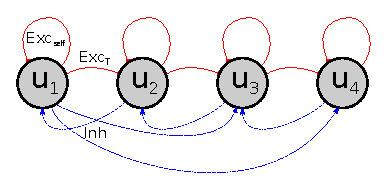
\includegraphics[scale=1.5]{diagram.eps}
\caption{The connectivity}\label{Fig:diagram}
\end{figure}


\subsection{A recall example}

\begin{figure}[h!]
\centering
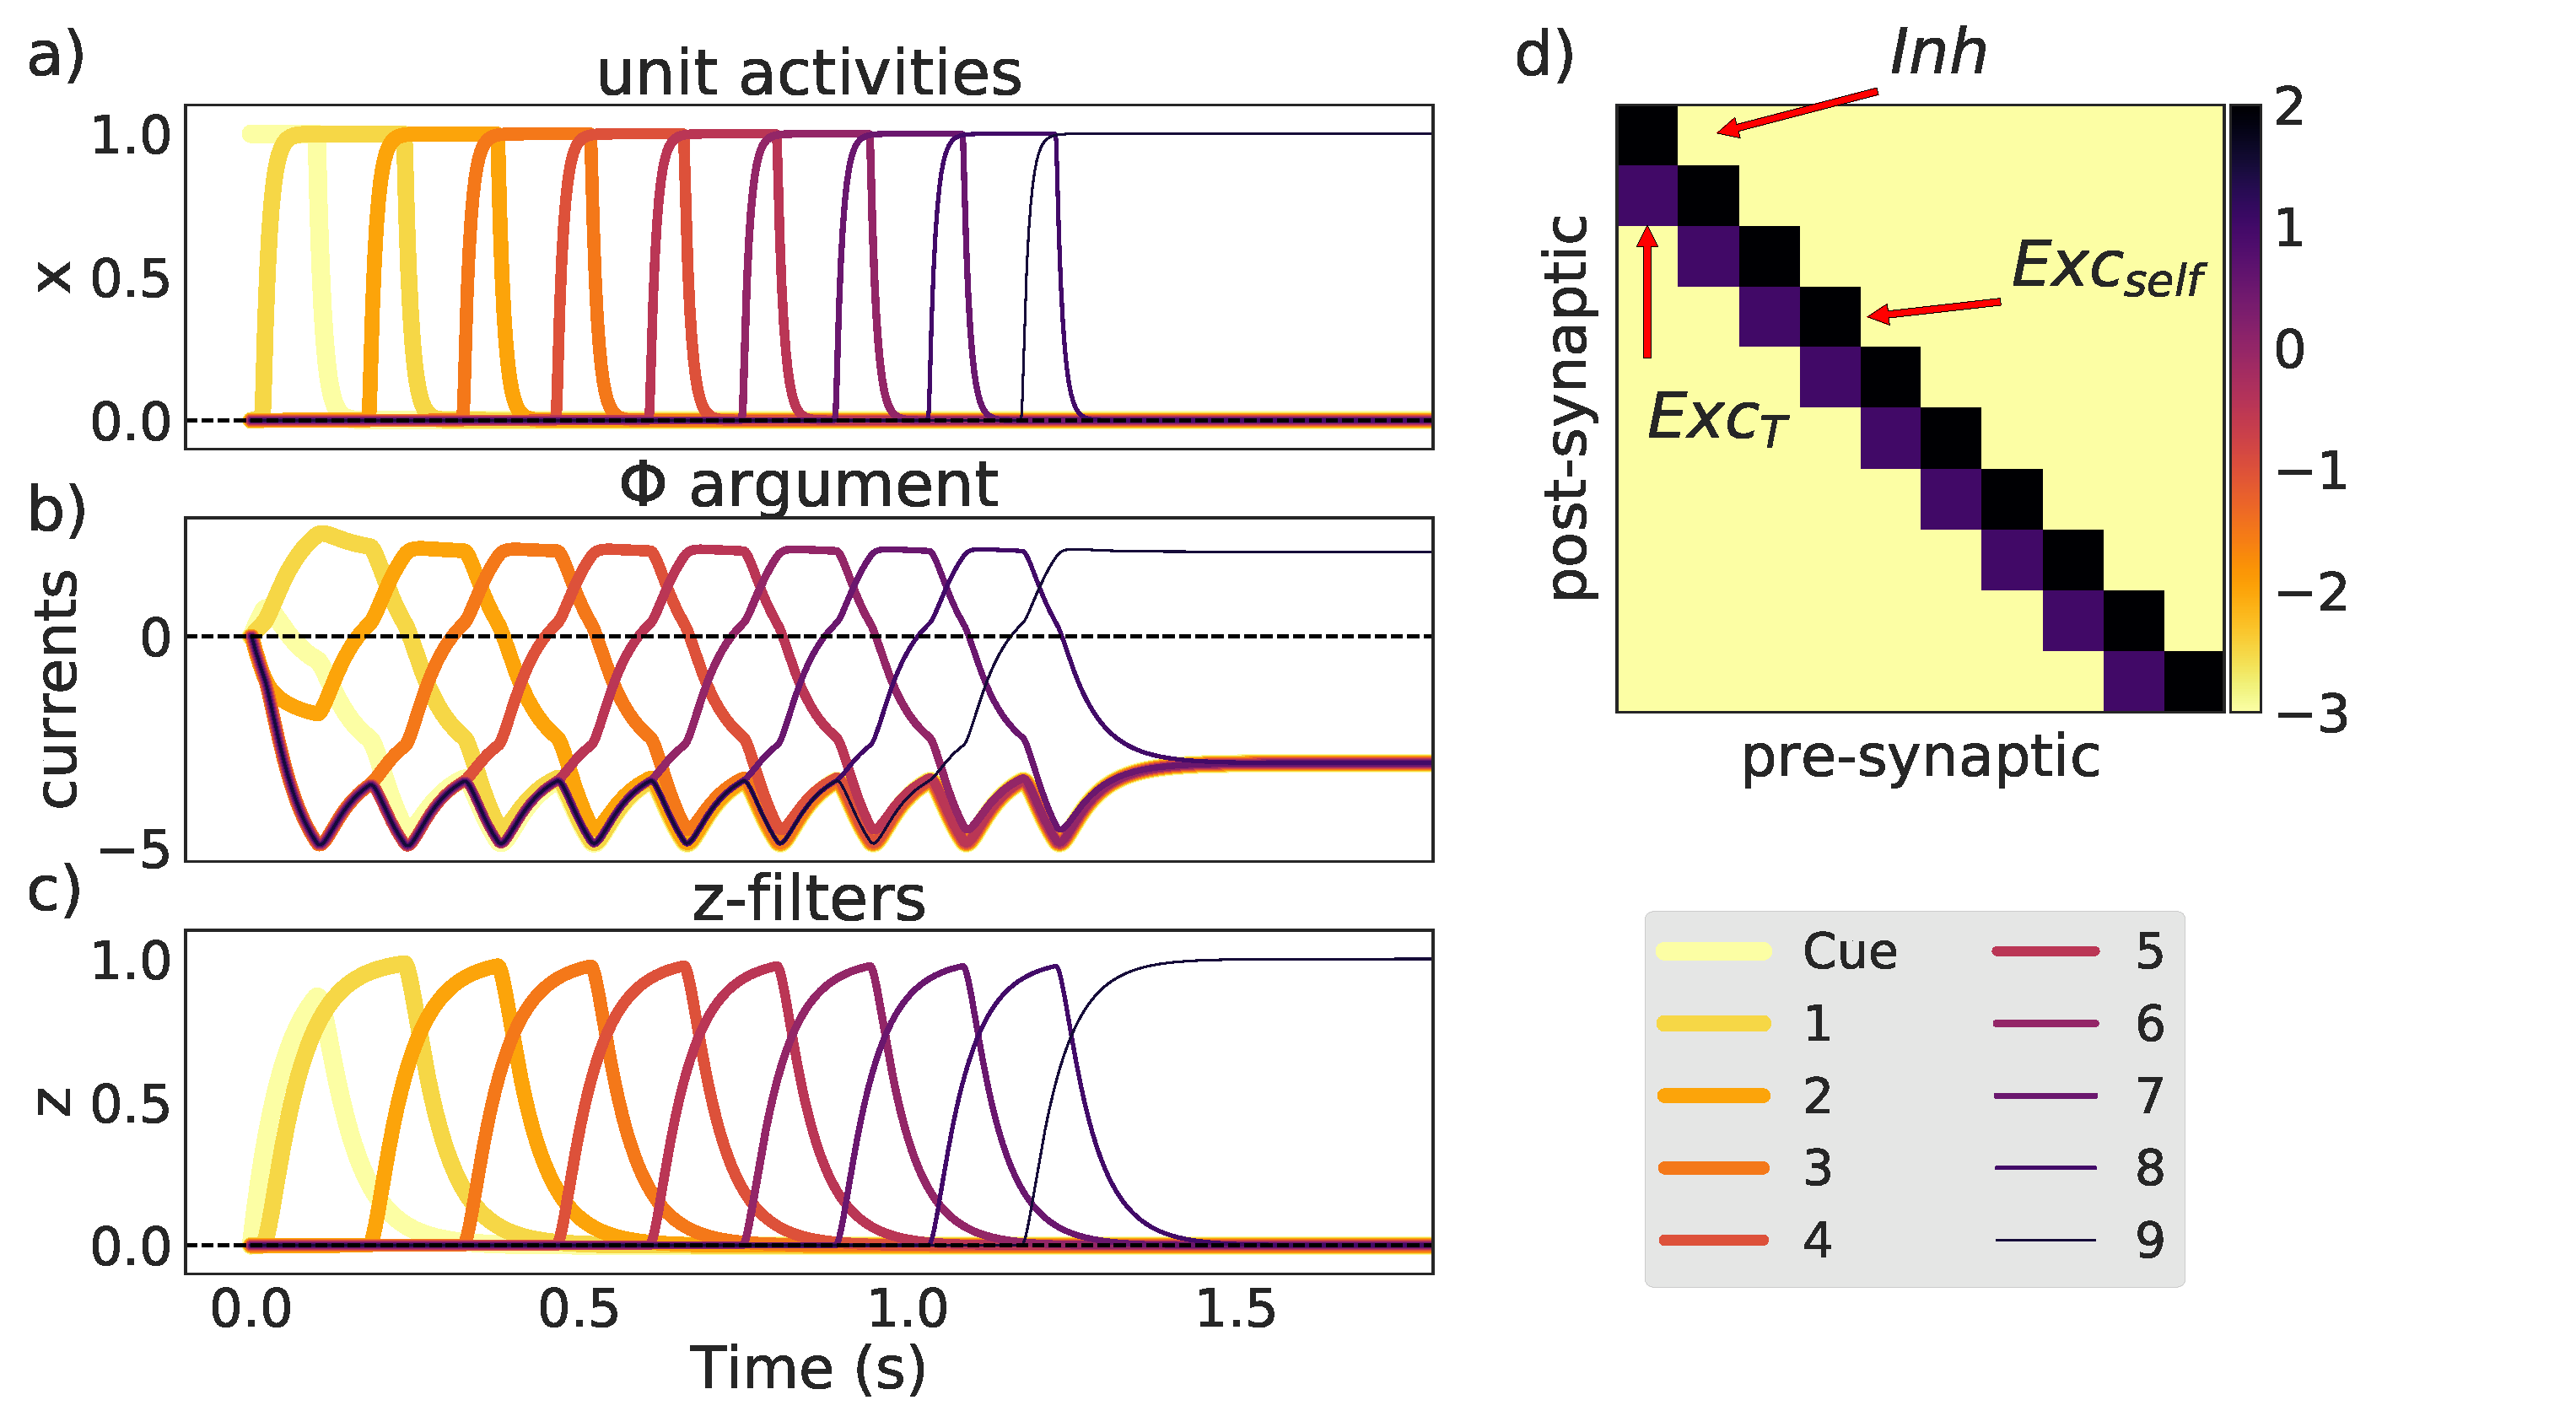
\includegraphics[scale=0.25]{recall.eps}
\caption{A recall example}\label{Fig:recall}
\end{figure}


\section{Dynamic Range}
\begin{figure}[h!]
\centering
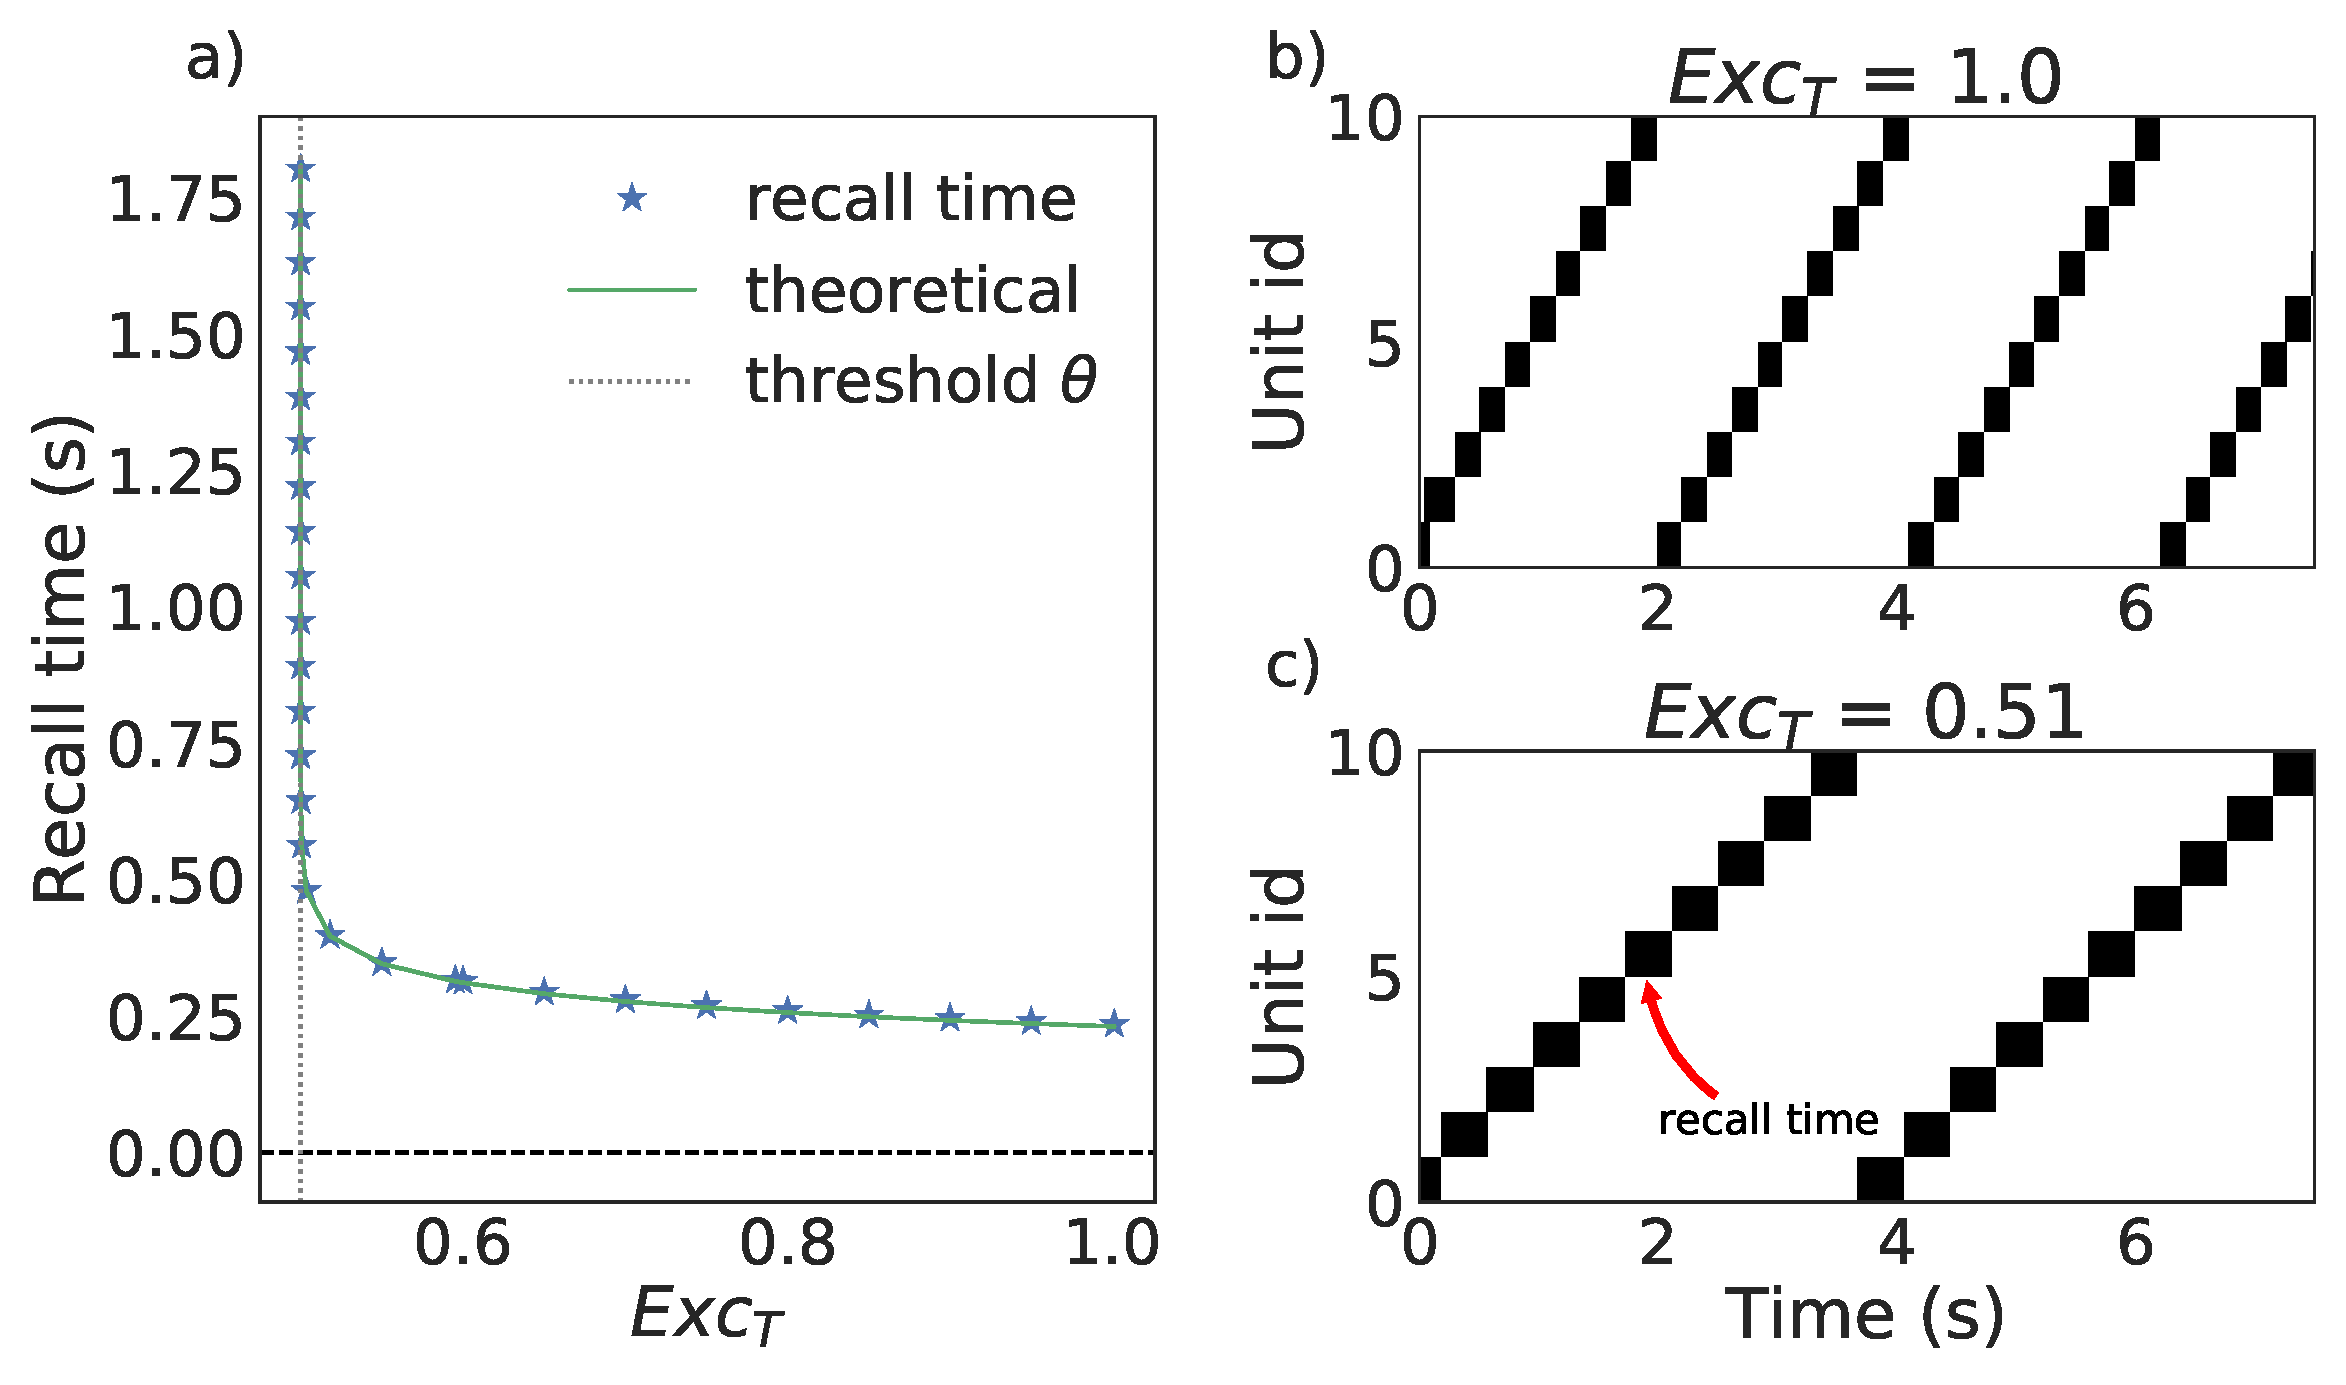
\includegraphics[scale=0.25]{dynamical_range.eps}
\caption{The dynamica range}\label{Fig:dynamical_range}
\end{figure}



\section{Learning Rule}

\begin{align}
\tau_w \dfrac{dw}{dt} &= (w_{max} - w) z_{pre}z_{post} + (w_{min} - w) (z_{post} - 1)z_{pre} 
\end{align}

\begin{figure}[h!]
\centering
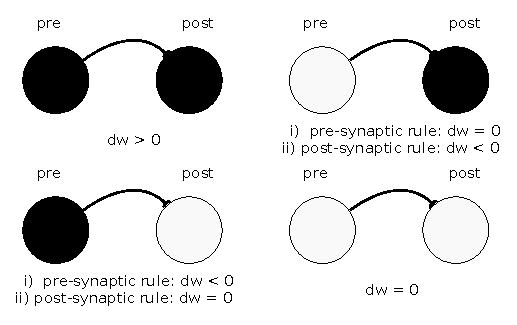
\includegraphics[scale=1.3]{plasticity_diagram.eps}
\caption{This is how plasticity works}\label{Fig:plasticity diagram}
\end{figure}


\begin{figure}[h!]
\centering
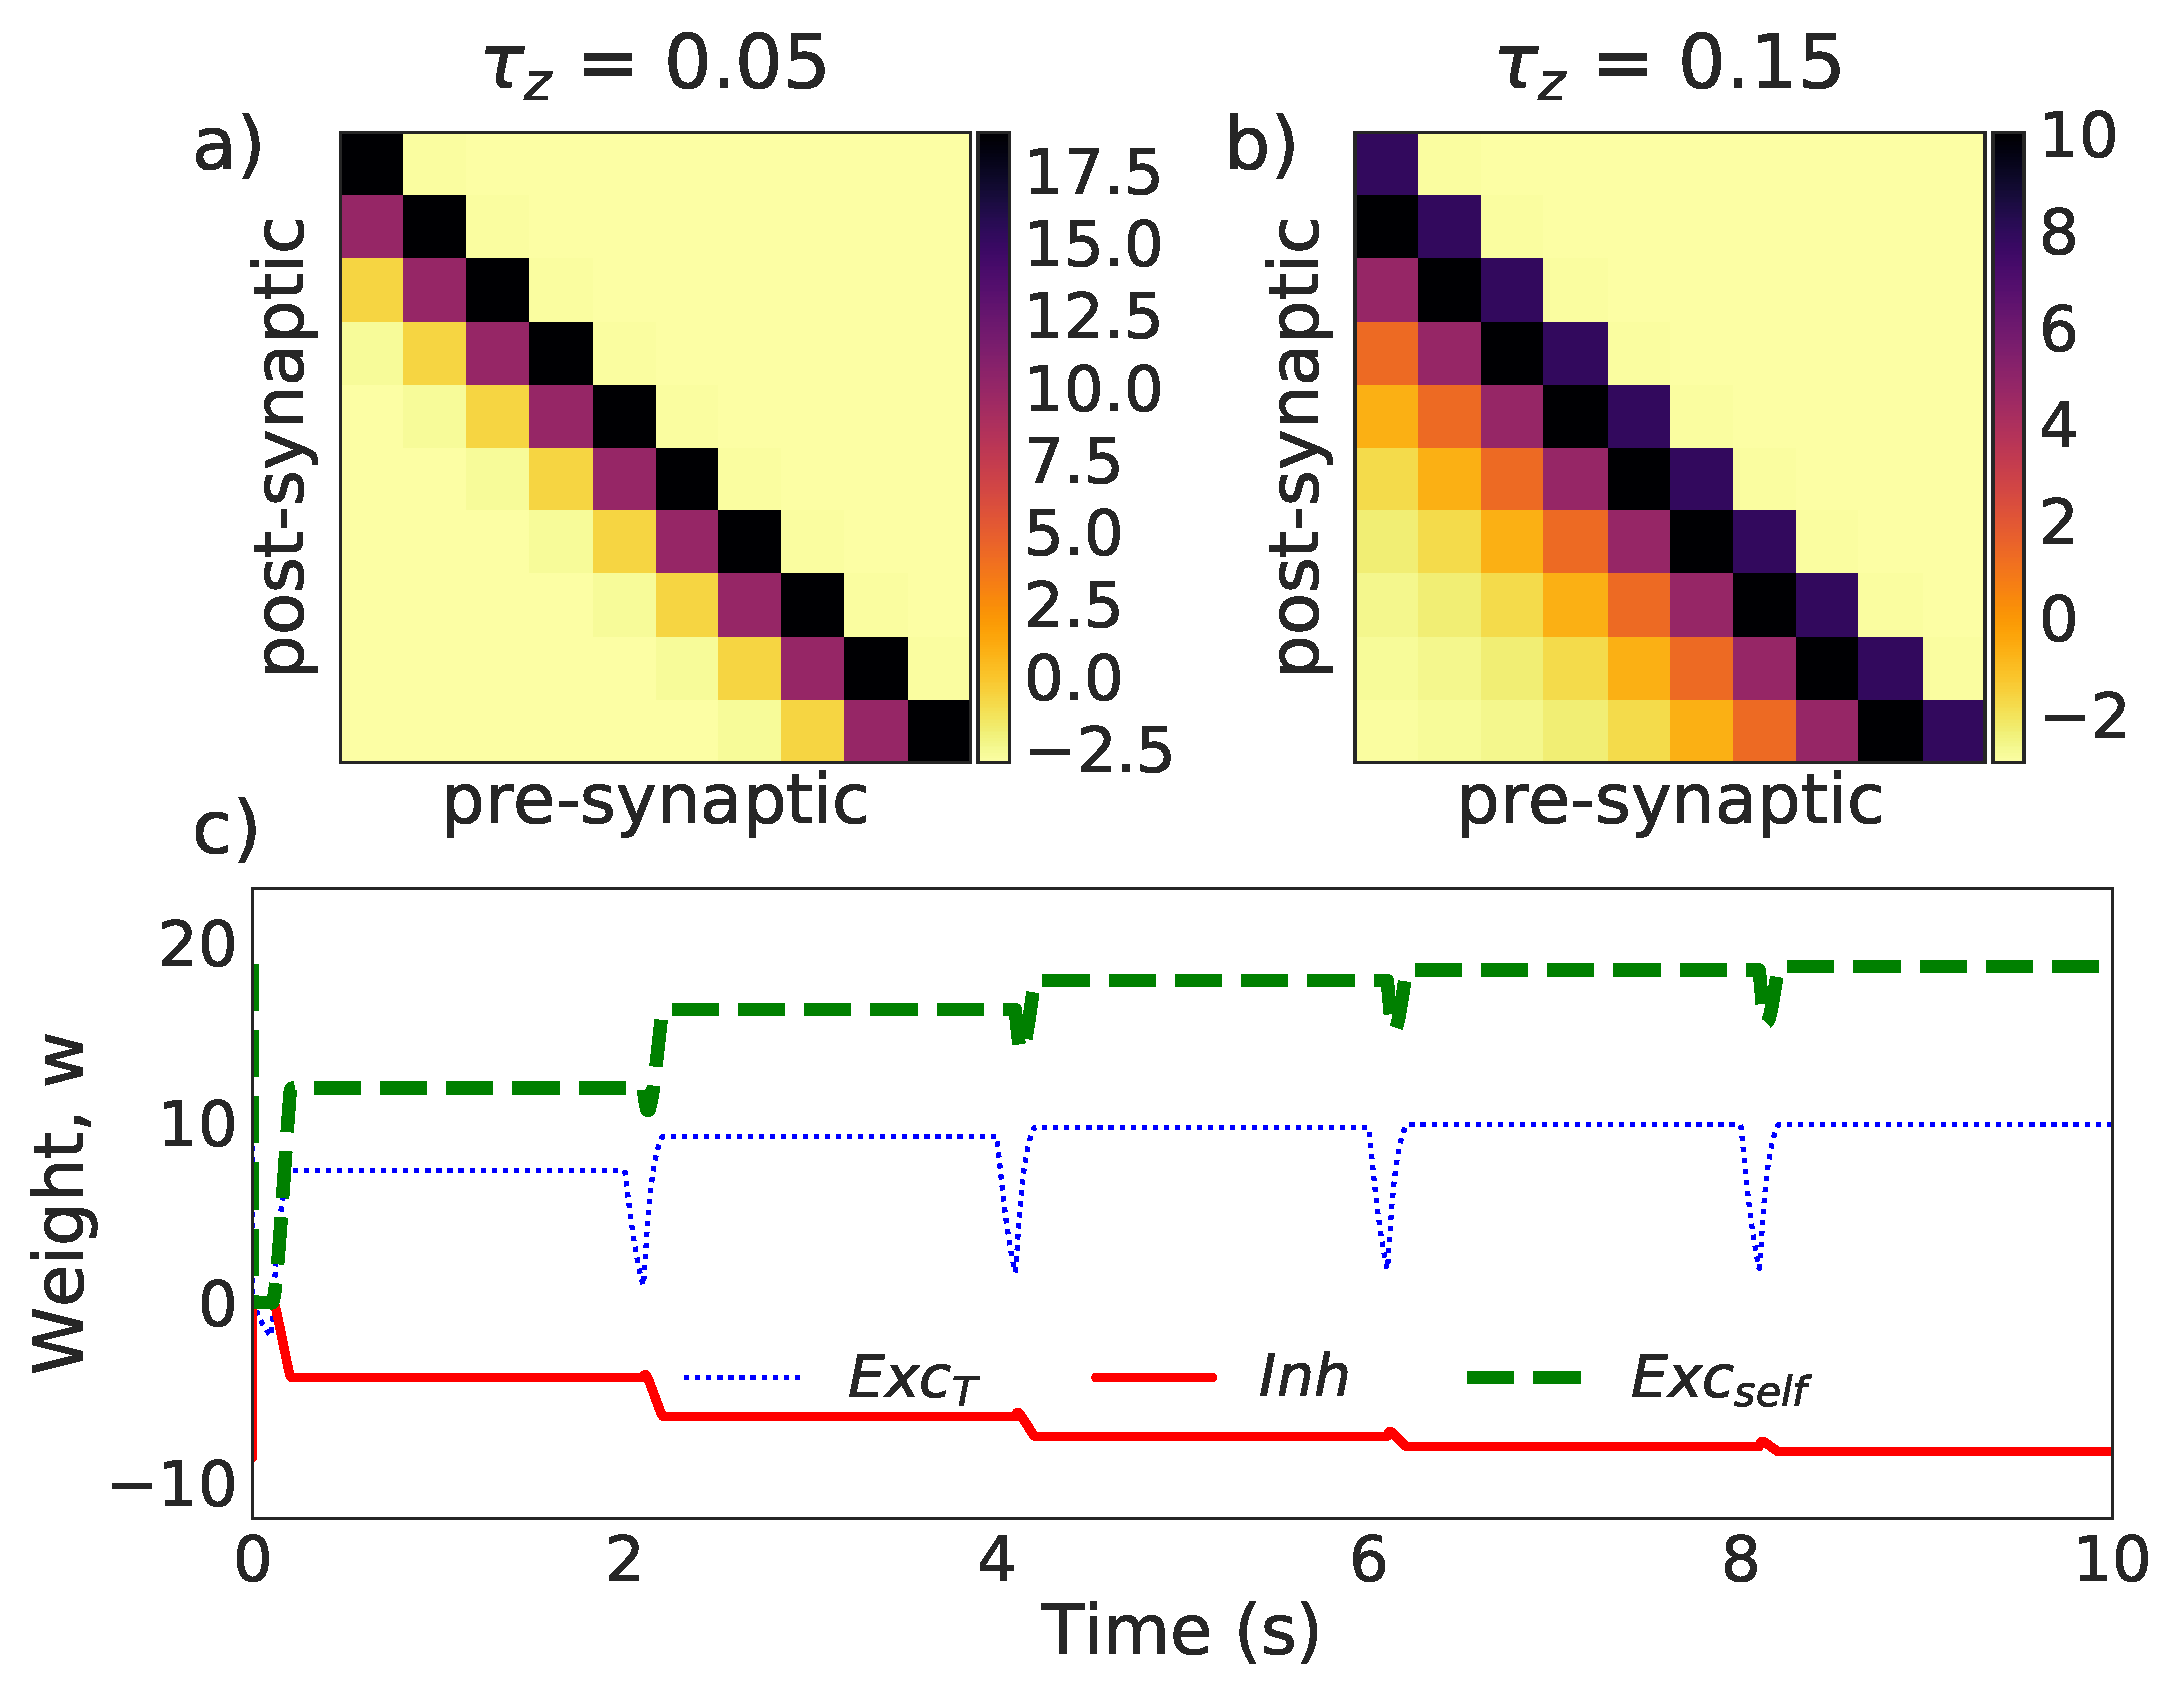
\includegraphics[scale=0.3]{training_rule.eps}
\caption{The training in action}\label{Fig:epochs}
\end{figure}


\begin{figure}[h!]
\centering
\includegraphics[scale=0.3]{training_rule_quantities.eps}
\caption{The dynamics of the learning rule}\label{Fig:learning_quantities}
\end{figure}

\textbf{Training time}
\begin{itemize}
\item  $Exc_{self}$: The longer the training time the longer the filter is activated with itself and therefore it grows. However
\item  $Inh$: W  
\end{itemize}

\section{Disambiguation}


\section{Discussion}

\section{Citation}
This ESANNV2.tex file defines how to insert references, both for
BiBTeX and non-BiBTeX users.  Please read the instructions in this
file.

% ****************************************************************************
% BIBLIOGRAPHY AREA
% ****************************************************************************

\begin{footnotesize}

% IF YOU DO NOT USE BIBTEX, USE THE FOLLOWING SAMPLE SCHEME FOR THE REFERENCES
% ----------------------------------------------------------------------------
\begin{thebibliography}{99}

% For books
\bibitem{Haykin_book} S. Haykin, editor. \emph{Unsupervised Adaptive Filtering vol.1 : Blind Source Separation}, John Willey ans Sons, New York, 2000.

% For articles
\bibitem{DelfosseLoubaton_article}N. Delfosse and P. Loubaton, Adaptibe blind separation of sources: A deflation
approach, \emph{Signal Processing}, 45:59-83, Elsevier, 1995.

% For paper in proceedings published as serie books (LNCS,...)
\bibitem{CrucCichAmari_bookproceedings} S. Cruces, A. Cichocki and S. Amari, The minimum entropy and cumulants based contrast functions for blind source extraction. In J. Mira and A. Prieto, editors, proceedings of the 6$^{th}$ \emph{international workshop on artificial neural networks} ({IWANN} 2001), Lecture Notes in Computer Science 2085, pages 786-793,
Springer-Verlag, 2001.

% For paper in conference proceedings
\bibitem{VrinsArchambeau_proceedings} F. Vrins, C. Archambeau and M. Verleysen, Towards a local separation performances estimator using common ICA contrast functions? In M. Verleysen, editor, \emph{proceedings of the $12^{th}$
European Symposium on Artificial Neural Networks} ({ESANN} 2004),
d-side pub., pages 211-216, April 28-30, Bruges (Belgium), 2004.

% For Technical Report
\bibitem{Stone_TechRep} J. V. Stone and J. Porrill, Undercomplete independent component analysis for signal separation and dimension
reduction. Technical Report, Psychology Department, Sheffield
University, Sheffield, S10 2UR, England, October 1997.
\end{thebibliography}
% ----------------------------------------------------------------------------

% IF YOU USE BIBTEX,
% - DELETE THE TEXT BETWEEN THE TWO ABOVE DASHED LINES
% - UNCOMMENT THE NEXT TWO LINES AND REPLACE 'Name_Of_Your_BibFile'

%\bibliographystyle{unsrt}
%\bibliography{Name_Of_Your_BibFile}

\end{footnotesize}

% ****************************************************************************
% END OF BIBLIOGRAPHY AREA
% ****************************************************************************

\end{document}
